% \usepackage{newfloat}
% \usepackage{listings}
% \usepackage{tcolorbox}
% \usepackage{lipsum}
% \usepackage{listings}
% \usepackage{courier}

% \newcommand{\theHalgorithm}{\arabic{algorithm}}
% % Define the style for the system prompt
% \DeclareCaptionStyle{ruled}{labelfont=normalfont,labelsep=colon,strut=off} % DO NOT CHANGE THIS
% \lstset{%
% 	basicstyle={\footnotesize\ttfamily},% footnotesize acceptable for monospace
% 	numbers=left,numberstyle=\footnotesize,xleftmargin=2em,% show line numbers, remove this entire line if you don't want the numbers.
% 	aboveskip=0pt,belowskip=0pt,%
% 	showstringspaces=false,tabsize=2,breaklines=true}
% \floatstyle{ruled}
% \newfloat{listing}{tb}{lst}{}
% \floatname{listing}{Listing}

\tcbset{
  colback=gray!10, % 背景颜色
  colframe=black, % 边框颜色
  fonttitle=\bfseries, % 标题字体
  sharp corners, % 直角边框
  boxrule=0.4mm, % 边框厚度
  top=2mm, bottom=2mm, left=6mm, right=0mm, % 内边距
  boxsep=0mm, % 内容与边框之间的距离
  width=\textwidth, % 盒子的宽度设置为页面宽度
}

\lstset{
  basicstyle=\ttfamily\scriptsize, % 基本字体样式和大小
  breaklines=true, % 自动换行
  backgroundcolor=\color{gray!10}, % 背景颜色
  frame=single, % 添加边框
  xleftmargin=2mm, xrightmargin=2mm, % 列表的左右边距
  aboveskip=0mm, belowskip=0mm, % 列表上下的垂直间距
  linewidth=\textwidth, % 列表的宽度设置为页面宽度
  escapeinside={(*@}{@*)} % 允许在 lstlisting 中使用 LaTeX 命令
}

\section{UE Environments}
\label{app:env}

\subsection{Comparison with other Simulators}
To better explain Table~\ref{tab:env_comparision}, we list the description of each symbol about the scene types and playable entities in Table~\ref{tab:symbol}. Since photorealism mainly relies on the engine used, we visualize the snapshots rendered by different engines in Figure~\ref{fig: visual_realism}. Note that Google Maps are images captured in the real world, but can not simulate the dynamic of the scenes and interactions between objects. By utilizing advanced rendering and physics engines, Unreal Engine simulates large-scale photorealistic environments that are not only visually appealing but also capable of complex interactions between agents and objects. So we choose to build environments on Unreal Engine.

\begin{table}[h]
\centering
\caption{The description of symbols used in Table~\ref{tab:env_comparision}.}
\vspace{-0.2cm}
\label{tab:symbol}
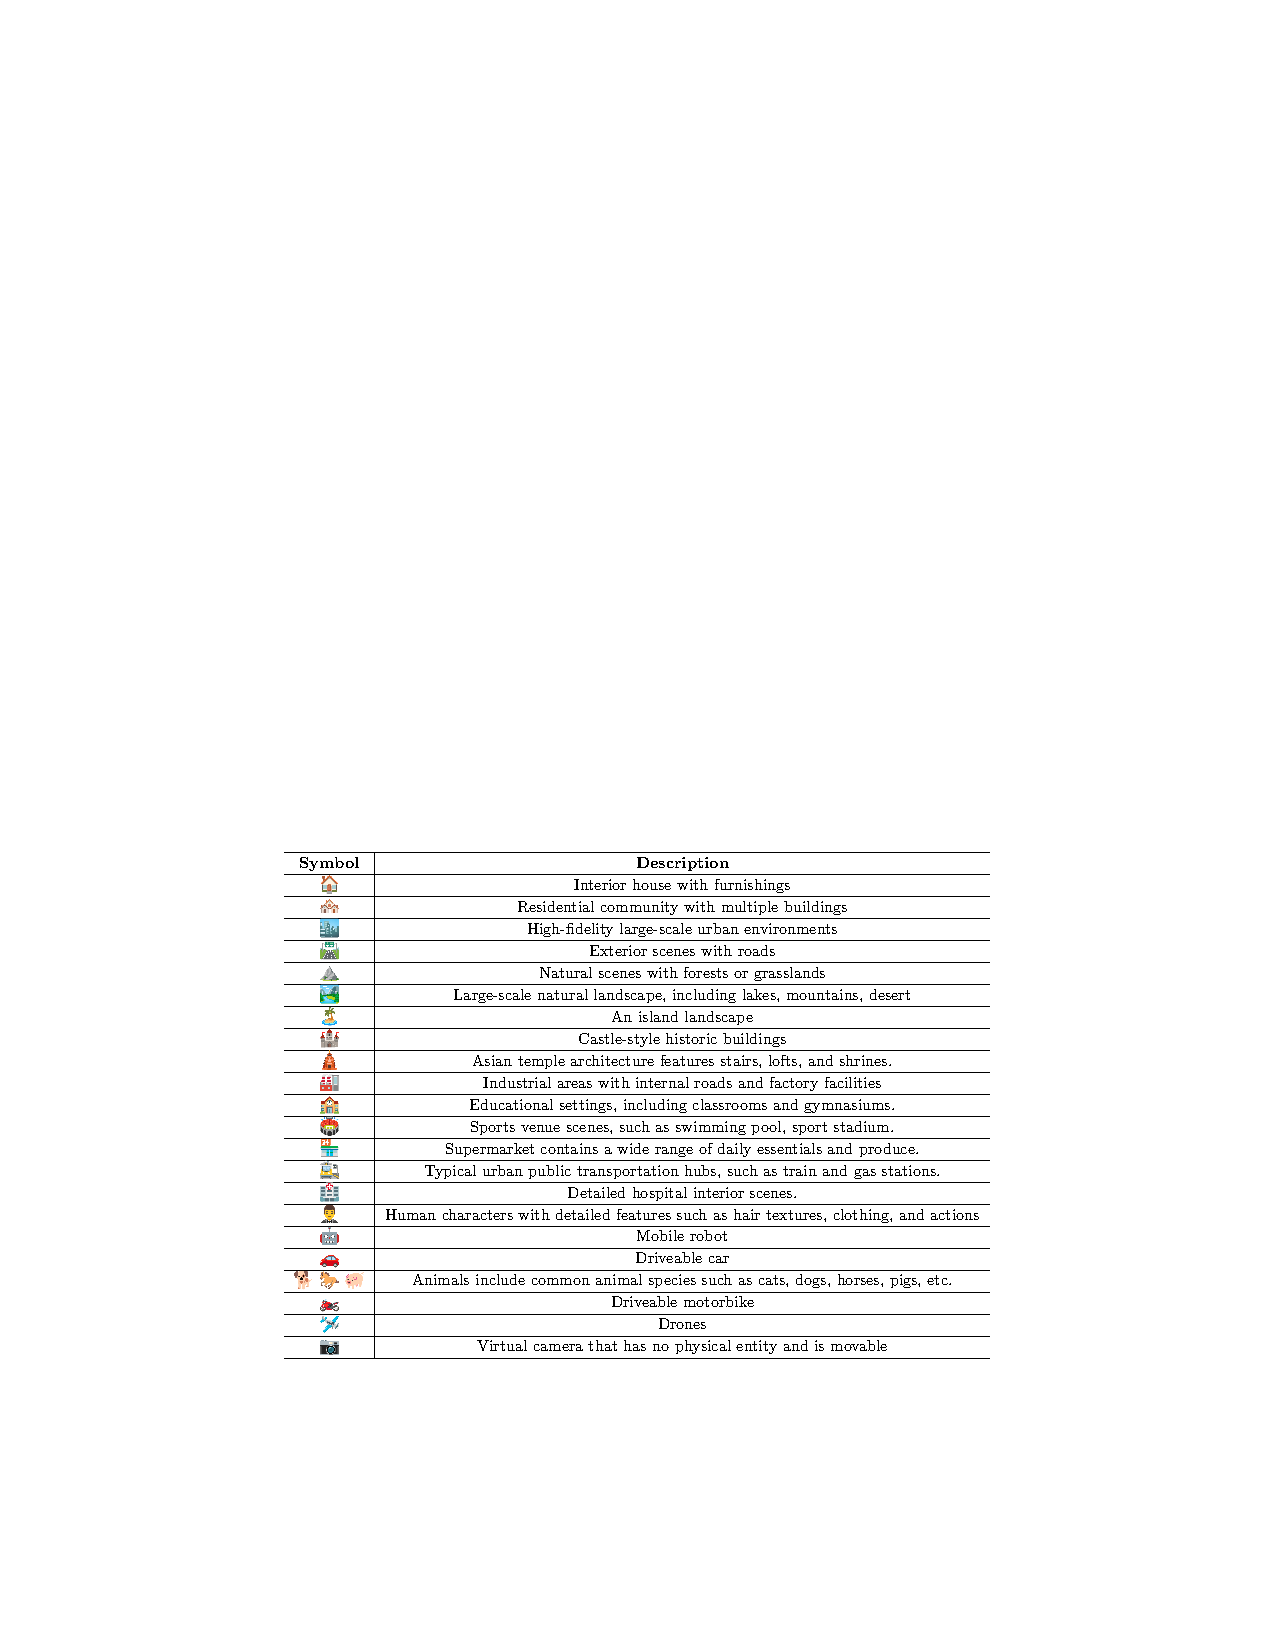
\includegraphics[width=0.9\linewidth]{image/emoji_description.pdf}
\end{table}


\begin{figure}[ht]
    \centering
    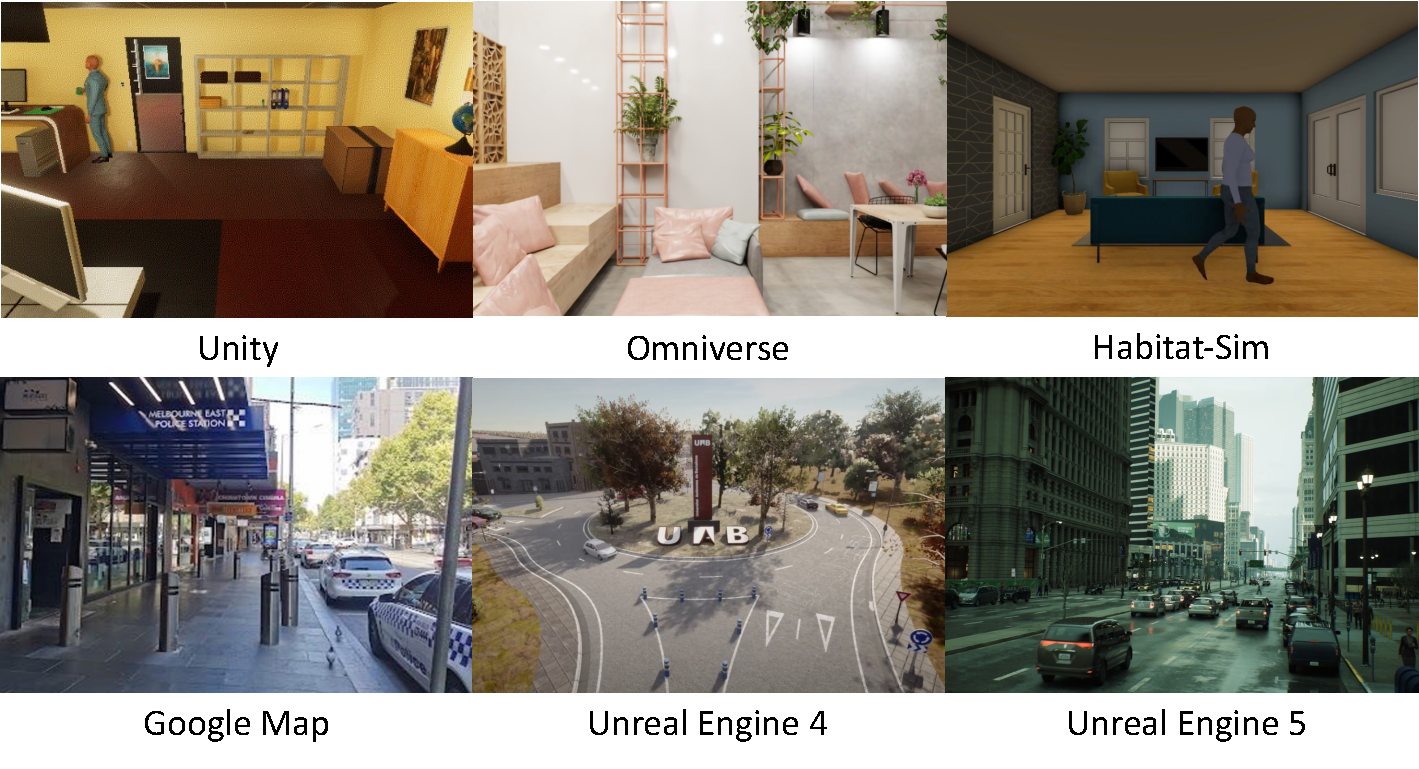
\includegraphics[width=0.9\linewidth]{image/visual_realism.pdf}
    \vspace{-0.3cm}
    \caption{Comparison of the visual realism of different engines: we show the snapshots captured from different engines to compare the photo-realism of different environments for an intuitive feeling. Note that Google Maps capture and reconstruct the images from the real world, but can not simulate the dynamic of the scenes and interactions between agents and objects.}
    \label{fig: visual_realism}
\end{figure}

\begin{figure}[t]
    \centering
    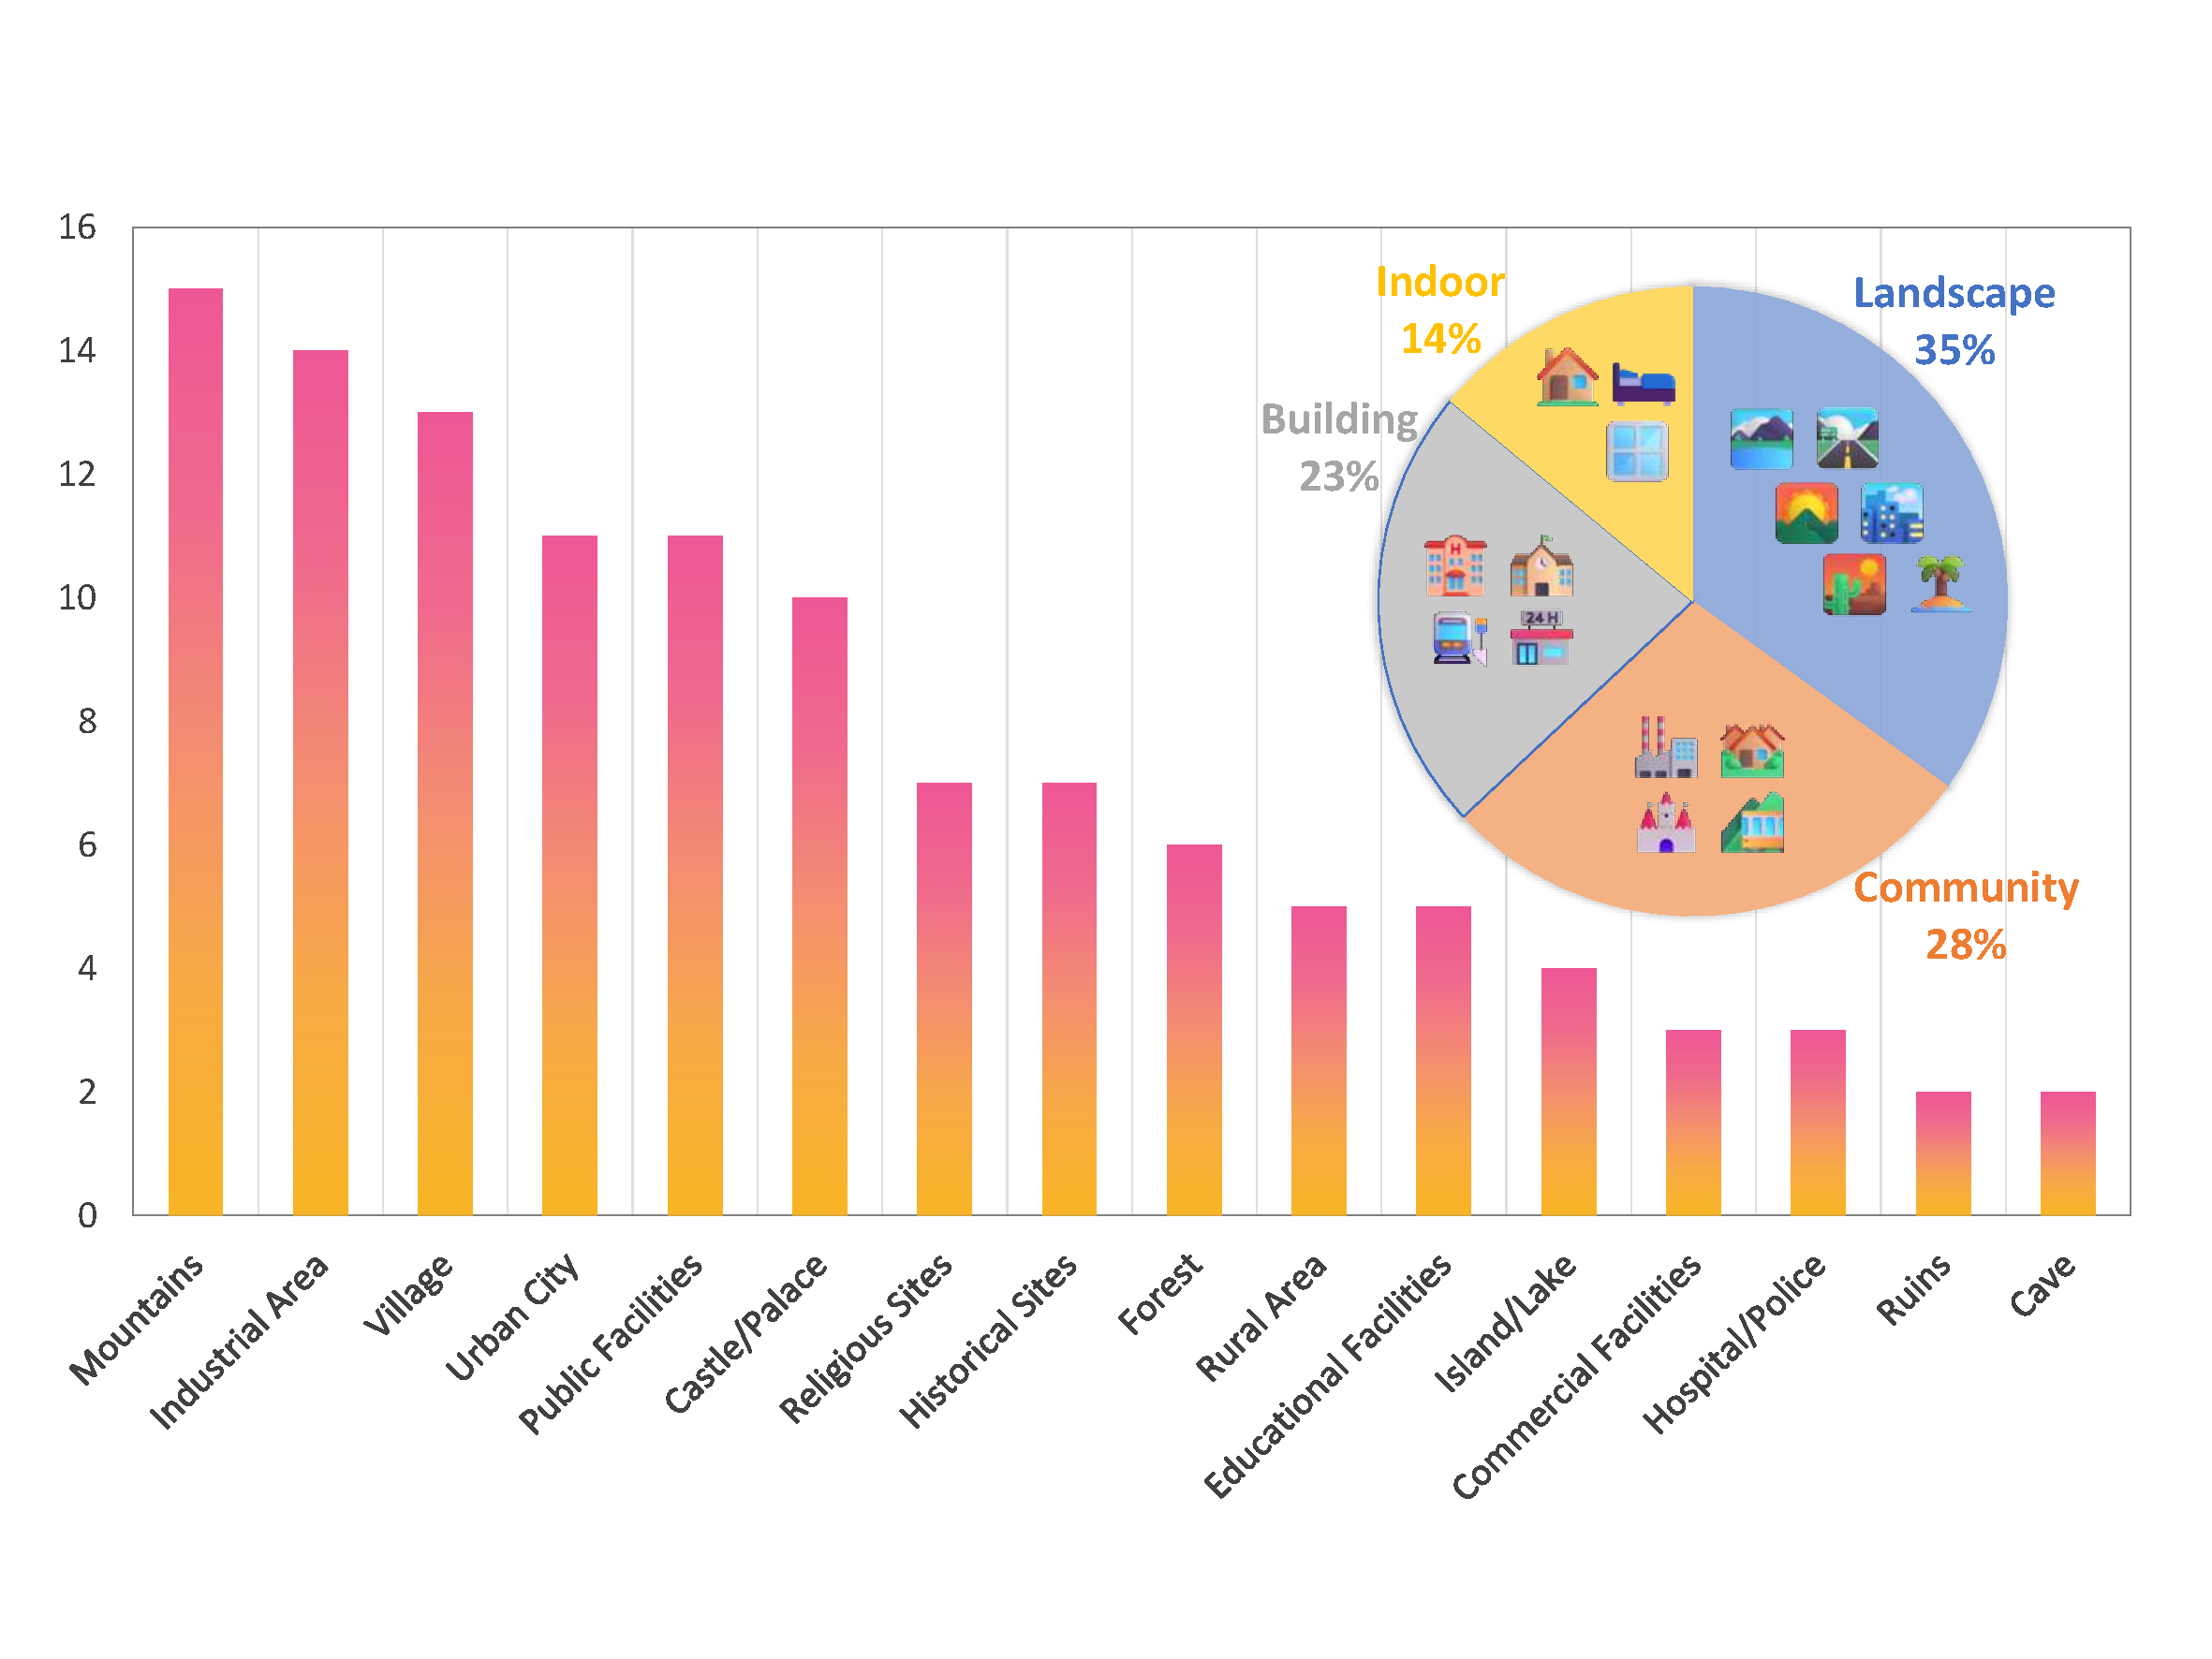
\includegraphics[width=1\linewidth]{image/stastic_full.pdf}
    \caption{The statistical distribution of scene content and scale in UnrealZoo. The bar chart depicts the number of scenarios featuring each type of content, noting that larger scenes may encompass multiple categories. The pie chart classifies these scenes by scale, revealing a predominance of large-scale `Landscape' environments, followed by `Community', `Building', and `Indoor' levels. The distribution reflects the diversity of UnrealZoo and the balanced composition of scenes of different scales. }
    \label{fig:stastic_distribution}
\end{figure}

\subsection{Environments used in Visual Navigation}
We carefully selected two photo-realistic environments (\textbf{Roof} and \textbf{Factory}) for training and evaluating navigation in the wild, shown in Figure~\ref{fig:Nav_env}. The Roof environment features multiple levels connected by staircases and large pipelines scattered on the ground, providing an ideal setting for the agent to learn complex action combinations for transitioning between levels, such as jumping, climbing, and navigating around obstacles. The Factory environment, on the other hand, is characterized by compact boxes and narrow pathways, challenging the agent to determine the appropriate moments to jump over obstacles or crouch to navigate under them. These two environments offer diverse spatial structures, enabling agents to develop an understanding of multi-level transitions and precise obstacle avoidance.

\begin{figure}[t]
    \centering
    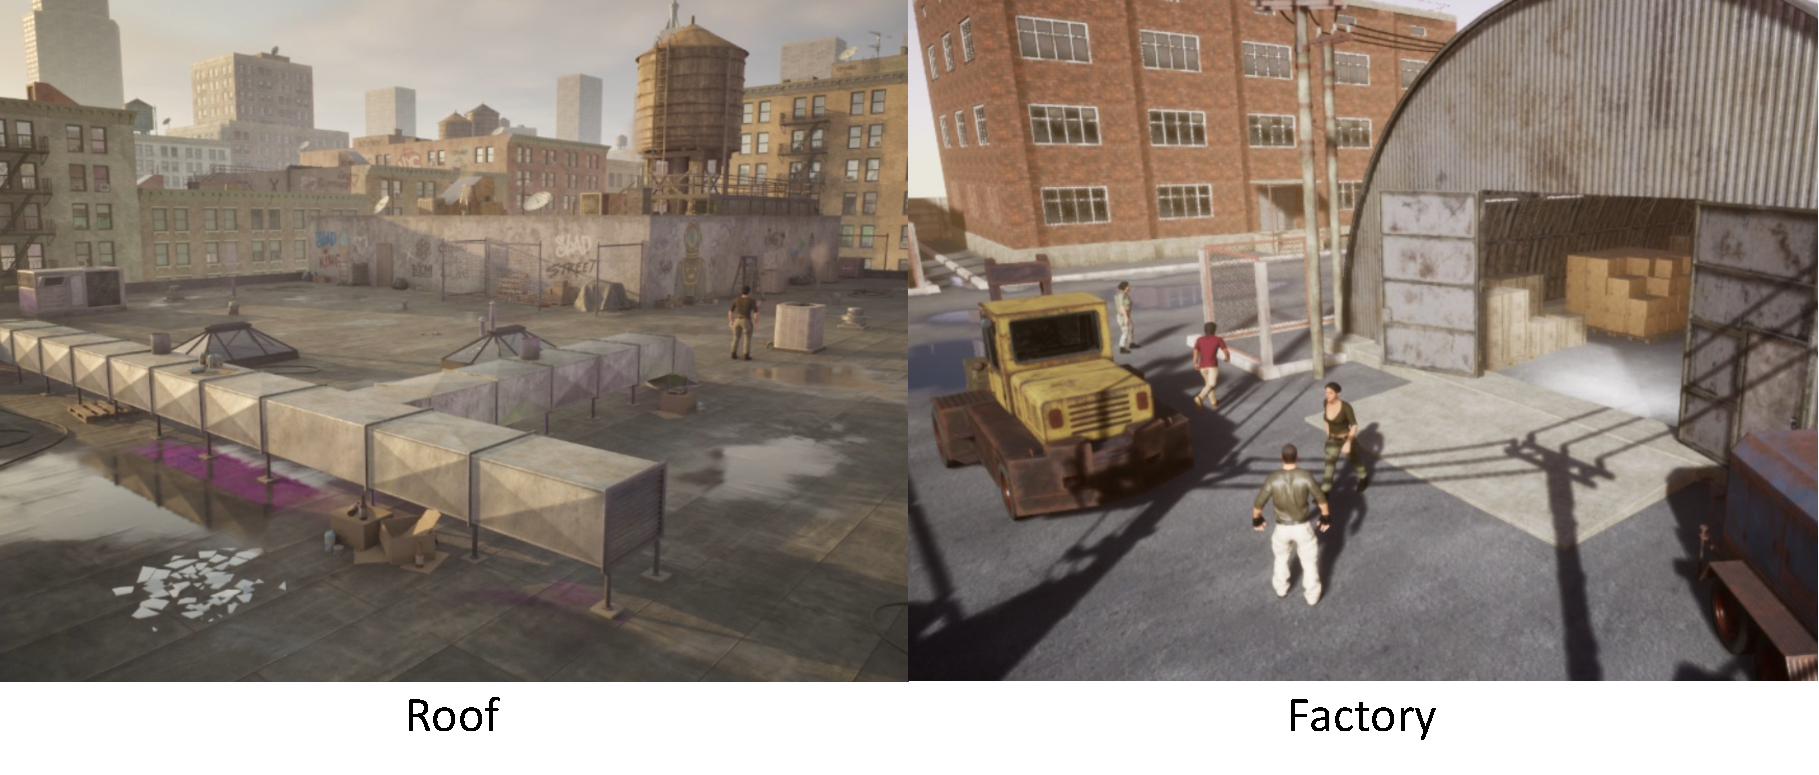
\includegraphics[width=0.8\linewidth]{image/Nav_env.pdf}
    \caption{ Two photo-realistic environments used for visual navigation. }
    \label{fig:Nav_env}
\end{figure}

% \subsection{Offline Data for Embodied Visual Tracking}

\subsection{Environments used in Active Visual Tracking}
\label{app:env_track}
For training agents via offline reinforcement learning, we selected 8 distinct environments to collect demonstrations, as is shown in Figure~\ref{fig:data_distribution}. 
To comprehensively evaluate the generalization of the active visual tracking agents, we selected \textbf{16} distinct environments, categorized into Interior Scenes, Palaces, Wilds, and Modern Scenes. Each category presents unique challenges: 1) \textbf{Interior Scenes} feature complex indoor structures with frequent obstacles; 2) \textbf{Palaces} include multi-level structures and narrow pathways; 3) \textbf{Wilds} encompass irregular terrain and varying illumination; 4) \textbf{Modern Scenes} offer high-fidelity, real-world scenarios with modern buildings and objects. These diverse environments facilitate a thorough assessment of the agent’s generalization capabilities across varying complexities. The snapshot of each environment is shown in Figure ~\ref{fig:eval_env}.

\begin{figure}[t]
    \centering
    \includegraphics[width=1\linewidth]{image/Environment_category.pdf}
    \caption{The snapshots of 16 environments used for testing active visual tracking agents. The text on the left indicates the category corresponding to that line of environment.}
    \label{fig:eval_env}
\end{figure}


\subsection{Navigation Mesh}
 Based on \href{https://dev.epicgames.com/documentation/en-us/unreal-engine/world-partitioned-navigation-mesh?application_version=5.4}{NavMesh}, we build an internal navigation system, allowing agents to autonomously navigate with the built-in AI controller in the Unreal Engine. This includes path-finding and obstacle-avoidance capabilities, ensuring smooth and realistic movement throughout diverse terrains and structures. Moreover, in our City style map, we manually construct road segmentation, we manually segment the roads to distinguish between pedestrian and vehicle pathways. When agents use the navigation system for autonomous control, they will navigate the shortest path based on the priority of the different areas. Figure~\ref{fig:nav_mesh} shows an example of the rendered semantic segmentation for NavMesh in an urban city.
 
\begin{figure}[t]
    \centering
    \includegraphics[width=0.8\linewidth]{image/navmesh.png}
    \caption{An example of the NavMesh with semantic segmentation. The human character will prioritize using the pink area for pedestrian navigation tasks, while the vehicles will use the blue area.}
    \label{fig:nav_mesh}
\end{figure}



\section{Exemplar Tasks}

\subsection{Visual Navigation}
\label{app:navigation_task}
In this task, the agent is initialized at a random location in the environment at the beginning of each episode, while the target object's location and category remain fixed throughout. The agent must rely on its first-person view observations and the relative spatial position of the target as input. The ultimate objective is to locate the target object within 2000 steps. Success is defined by the agent reducing the relative distance to less than 3 meters and aligning its orientation such that the relative rotation between the target and the agent is smaller than 30 degrees (in the front of the agent). This setup challenges the agent to optimize its movements and decision-making while adapting to the randomized starting conditions and dynamic environment. All methods in the task share the same discrete action space to control the movement, consisting of moving forward (+1 meter/s), moving backward (-1 meter/s), turning left (-15 degrees/s), turning right (+15 degrees/s), jumping (two continuous jumping actions trigger the climbing action), crouching, and holding position. This action space enables the agent to navigate and interact with complex 3D environments, making strategic decisions in real-time to reach the target object efficiently. The step reward for the agent is defined as:
\begin{equation}
    r(t) = \tanh ( \frac{dis2target(t-1)-dis2target(t)}{max(dis2target(t-1),300)} - \frac{|Ori|}{90 ^{\circ}} )
\end{equation}
where $dis2target(t)$ is the Euclidean distance between the agent and the target at a given timestep $t$ and $|Ori|$ is the absolute orientation error (in degrees) between the agent's current heading and the direction toward the target, normalized by $90^{\circ}$
\subsection{Active Visual Tracking}
\label{app:tracking_task}
Referring to previous works \citep{zhong2024empowering}, we use human characters as an agent player and a continuous action space for agents. The action space contains two variables: the angular velocity and the linear velocity. Angular velocity varies between $-30^{\circ}/s$ and $30^{\circ}/s$, 
while linear velocity ranges from $-1\ m/s$ to $1\ m/s$. In the agent-centric coordinate system, the reward function is defined as:
\begin{equation}
    r = 1- \frac{\vert\rho - \rho^*\vert}{\rho_{max}} - \frac{\vert\theta-\theta^*\vert}{\theta_{max}}
\end{equation}
where $(\rho, \theta)$ denotes the current target position relative to the tracker, $(\rho^*, \theta^*)=(2.5m, 0)$ represents the expected target position, i.e., the target should be $2.5m$ in front of the tracker. The error is normalized by the field of the view $(\rho_{max}, \theta_{max})$. During execution, an episode ends with a maximum length of 500 steps, applying the appropriate termination conditions. In the experiment, we adopt the original neural network structure and parameters, as listed in Table ~\ref{offline_tracking_agent} and ~\ref{tab:HyperParam_offline}. 

\begin{figure}[t]
    \centering
    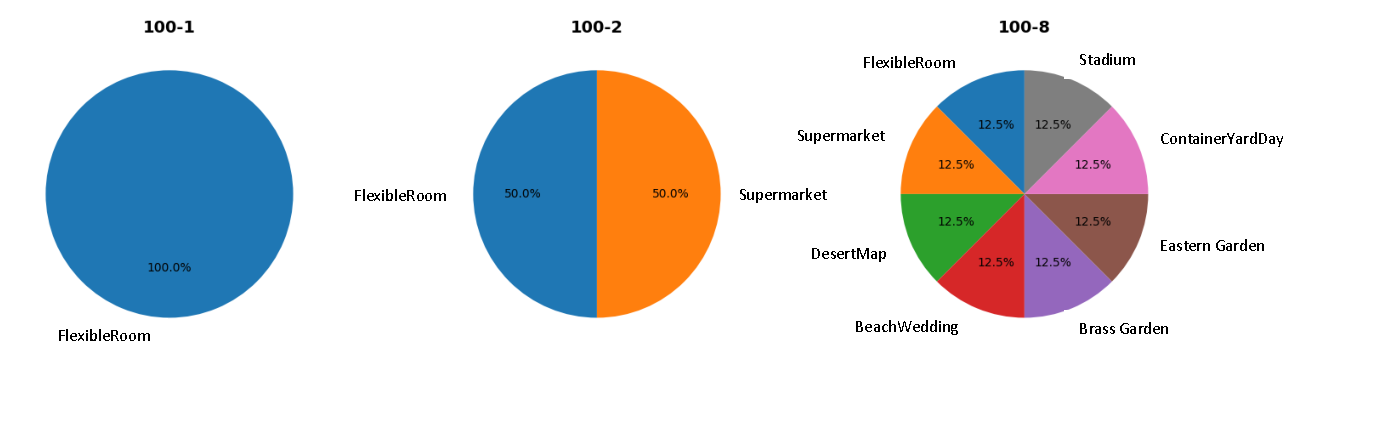
\includegraphics[width=1\linewidth]{image/data_distribution.pdf}
    \vspace{0.1cm} % 调整主图与子图之间的间距
    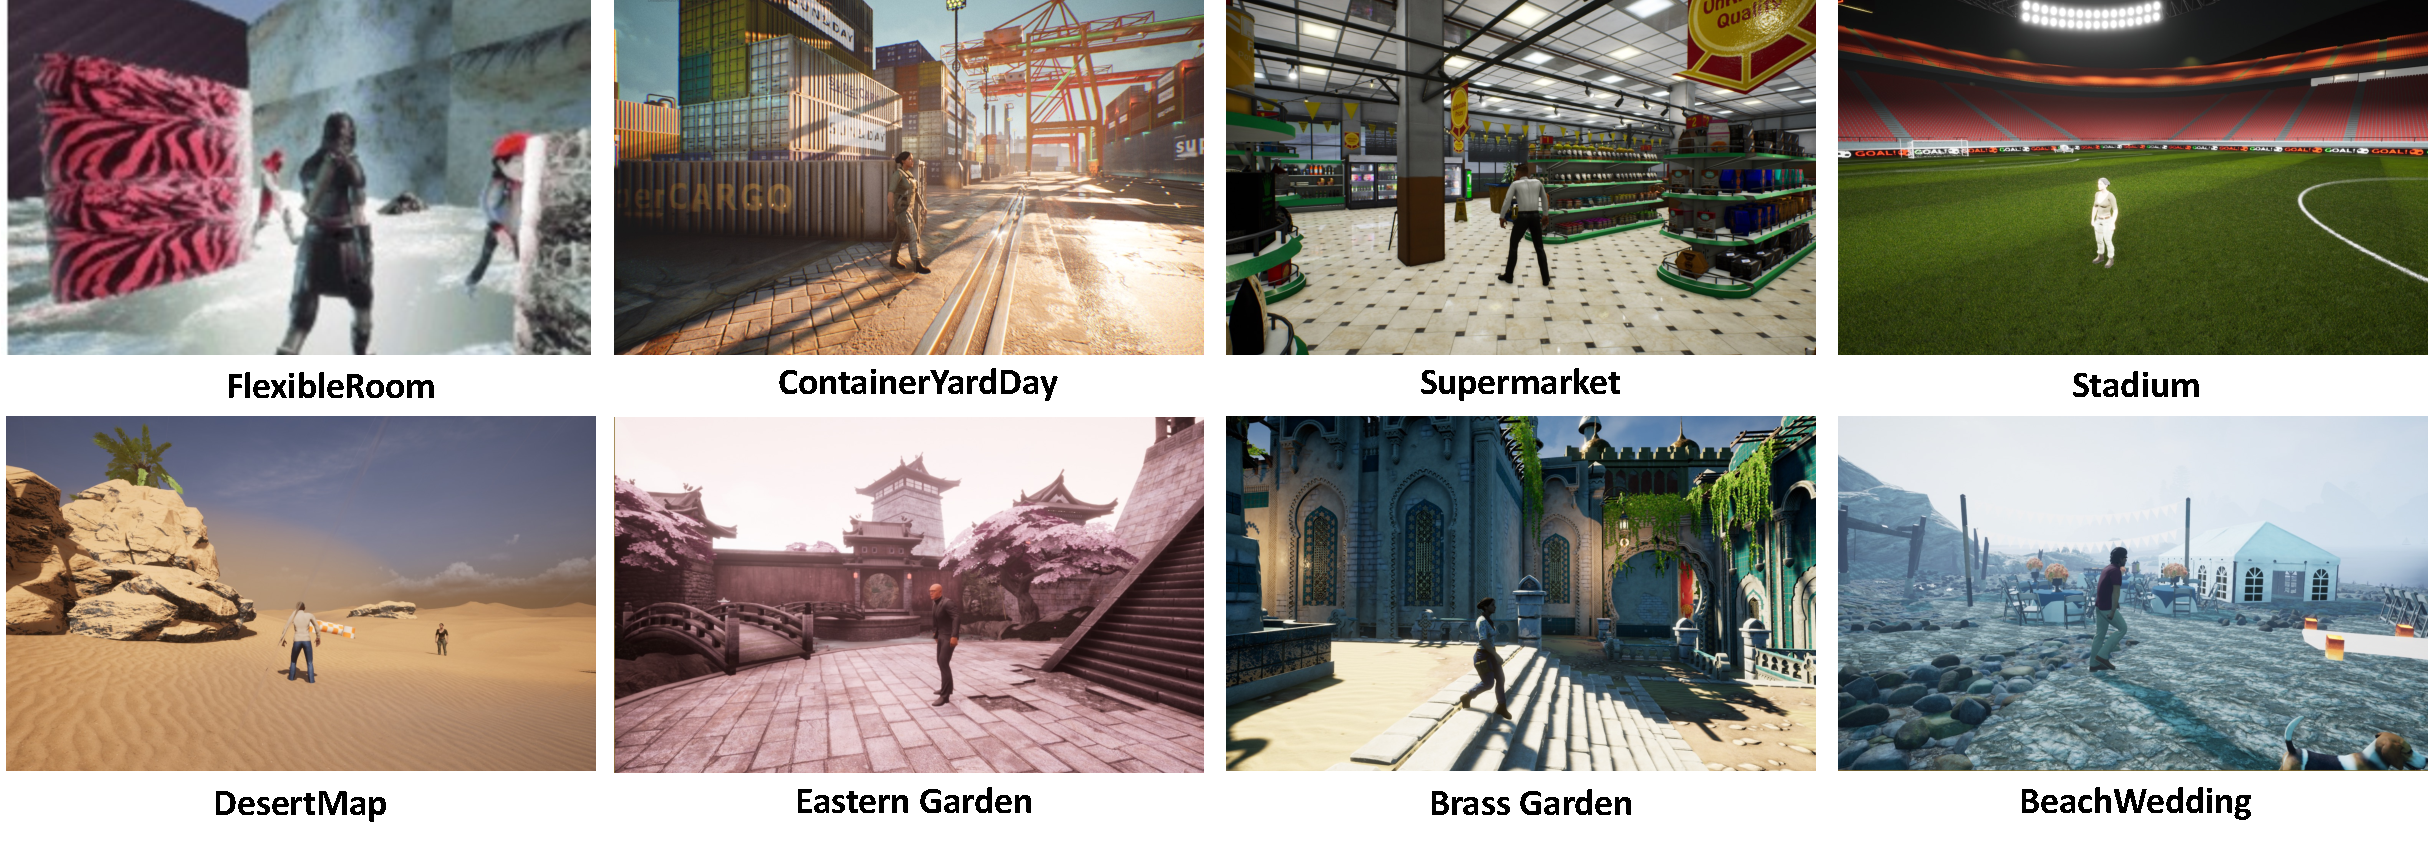
\includegraphics[width=1\linewidth]{image/training_env.pdf}
    \caption{The 8 environments used for collecting offline dataset.}
    \label{fig:data_distribution}
\end{figure}

\subsection{Task Configuration In a JSON File}
We provide an example of the task configuration JSON file in Figure~\ref{app:json}. Using the JSON file, we can easily set the configuration of the binary, the continuous and discrete action space for each agent, the placement of the binding camera, choose the area to reset, and other hyper-parameters about the environments.

\begin{figure*}[t]
  \centering

\begin{tcolorbox}[title= A Json File for Task Configuration ]
\begin{lstlisting}[texcl=true, escapechar=|]
    "env_name": env_name,
    "env_bin":path-to-binary,
    "env_map": map_name,
    "env_bin_win": path-to-binary(for windows),
    "third_cam": {"cam_id": 0,"pitch": -90,"yaw": 0,"roll": 0,"height_top_view": 1460.0,"fov": 90},
    "height": 460.0,
    "interval": 1000,
    "agents": {
        "player": {
            "name": ["BP_Character_923"],
            "cam_id": [3],
            "class_name": ["bp_character_C"],
            "internal_nav": true,
            "scale": [1,1,1],
            "relative_location": [20,0,0],
            "relative_rotation": [ 0,0,0],
            "head_action_continuous": {"high": [15,15,15], "low": [-15,-15,-15]},
            "head_action": [ [0,0,0],[0,30,0],[0,-30,0]],
            "animation_action": ["stand","jump","crouch"],
            "move_action": [
            [angular, velocity]
                ...
            ],
            "move_action_continuous": {"high": [30,100],"low": [-30,-100]}
        },
        "animal": {
            "name": ["BP_animal_2"],
            "cam_id": [1],
            "class_name": ["BP_animal_C"],
            "internal_nav": true,
            "scale": [1,1,1],
            "relative_location": [20,0,0],
            "relative_rotation": [0,0,0],
            "move_action": [
                [angular, velocity]
                ...
            ],
            "move_action_continuous": { "high": [30,100],"low": [-30,-100]}
        },
        "drone": {
            "name": ["BP_Drone01_2"],
            "cam_id": [2],
            "class_name": ["BP_drone01_C"],
            "internal_nav": false,
            "scale": [ 0.1,0.1,0.1],
            "relative_location": [0,0,0],
            "relative_rotation": [0,0,0],
            "move_action": [
              [angular, velocity]
                ...
            ],
            "move_action_continuous": {"high": [1,1,1,1],"low": [-1,-1,-1,-1]}
        }
    },
    "safe_start": [
        [x,y,z],
        ...
    ],
    "reset_area": [x_min,x_maxin,y_min,y_max,z_min,z_max],
    "random_init": false,
    "env": {"interactive_door": []},
    "obj_num": 466,
    "size": 192555.0,
    "area": 9900.0,
    "bbox": [110.0, 90.0,19.45]
    
\end{lstlisting}
\end{tcolorbox}
  \caption{An example of the task configuration file in JSON format.}
    \label{app:json}
  \label{figure:task_json}
\end{figure*}

% \section{Offline Datasets}
\subsection{Collecting Demonstration for Active Visual Tracking}
To demonstrate the flexibility of the environment, we use state-based expert policy and the multi-level perturbation strategy ~\citep{zhong2024empowering} to automatically generate various imperfect demonstrations as the offline dataset. 
For active visual tracking, we employ three distinct datasets for training agents via offline reinforcement learning (Offline RL) algorithms, referred to as \textit{1 Env.}, \textit{2 Envs.}, and \textit{8 Envs}. The detailed composition of each dataset is depicted in Figure~\ref{fig:data_distribution}. For the \textit{1 Env.} dataset, we use only the FlexibleRoom, an abstract environment enriched with diverse augmentation factors, to gather 100k steps of trajectory data. For 2 Envs., we collect 50k step trajectories from FlexibleRoom and an additional 50k steps from the Supermarket environment. The 8 Envs. dataset involves eight different environments, with 12.5k steps collected from each. Therefore, \textbf{the total amount of data in the three datasets is the same (100k) to ensure the fairness of the comparison.}
These dataset configurations aim to highlight the critical role of environment diversity in enhancing the generalization capabilities of embodied AI agents.

\section{Implementation Details of Agents}

\subsection{RL-based Agents}
\label{app:onlineRL}
% algorithms, network architecture, hyper-parameters.
\textbf{Learning to navigate with online reinforcement learning.} For navigation, we construct an RL-based end-to-end model, using A3C~\citep{mnih2016asynchronous} to accelerate online reinforcement learning in a distributed manner. The model's structure is as follows: a mask encoder extracts spatial visual features from the segmentation mask, which are then passed to a temporal encoder to capture latent temporal information. Finally, the spatiotemporal features, concatenated with the target's relative spatial position, are fed into the actor-critic network to optimize the actor layer for action prediction. The detailed network structure and parameters used in the experiment are listed in Table ~\ref{RL-Based} and ~\ref{tab:HyperParam_nav}. Here, we provide the training curves in \textit{Roof} and \textit{Factory} environments, depicted in Figure~\ref{fig:training_curve}. In the \textit{Factory}, we set the number of workers to 4, while in the \textit{Roof}, the number of workers is set to 6. It can be observed that, for Online RL, the number of workers and the complexity of environments have a significant impact on training efficiency. Looking forward, we anticipate that offline-based algorithms can effectively address the challenges of training efficiency and generalization. 

\begin{table}[ht]
\centering
\caption{Details the neural network structure of RL-based agent for navigation task, where 5$\times$5-32S1 means 32 filters of size 5$\times$5 and stride 1, FC256 indicates the fully connected layer with output dimension 256, and LSTM128 indicates that all the sizes in the LSTM unit are 128.}
\begin{tabular}{c|c|c|c|c|c|c|c|c}
\hline\hline
Module & \multicolumn{8}{|c}{Mask Encoder}\\ \hline
Layer\# & CNN &Pool& CNN &Pool& CNN &Pool& CNN &Pool \\ \hline
Parameters &     5$\times$5-32\emph{S}1 &2-S2& 5$\times$5-32\emph{S}1 &2-S2& 4$\times$4-64\emph{S}1 &2-S2& 3$\times$3-64\emph{S}1 &2-S2  \\ \hline \hline
Module & \multicolumn{2}{|c|}{Temporal Encoder} &\multicolumn{3}{|c|}{ Actor} & \multicolumn{3}{|c}{Critic} \\ \hline
 Layer\# & FC& LSTM & \multicolumn{3}{c|}{FC}& \multicolumn{3}{c}{FC} \\ \hline
 Parameters &256 &128& \multicolumn{3}{c|}{2}&\multicolumn{3}{c}{2} \\ 

 \hline
\end{tabular}
\label{RL-Based}
\end{table}

\begin{table}[ht]
    \centering
     \caption{The experiment setting and hyper-parameters used for training the RL-based navigation agent.}
   \begin{tabular}{l|c|l|c}
\hline\hline
Name & Value &Name & Value \\ \hline
Learning Rate   & 1e-4 &LSTM update step & 20 \\ \hline
workers (Roof)   & 6 &LSTM Input Dimension& 256 \\ \hline
workers (Factory)  & 4 &LSTM Output Dimension& 128\\ \hline
% Image input size  &  160x160 \\ \hline
 Position Input Dimension & 2 &LSTM Hidden Layer size & 1 \\ \hline
 
% LSTM update step                    & 20 \\ \hline
% LSTM Input Dimension               & 256 \\ \hline
% LSTM Output Dimension               & 128 \\ \hline
% LSTM Hidden Layer size              & 1 \\ \hline
\end{tabular}
   
    \label{tab:HyperParam_nav}
\end{table}


\textbf{Learning to track with offline reinforcement learning.} For the tracking task, we adopt an offline reinforcement learning (Offline RL) approach to enhance training efficiency and improve the agent's generalization to unknown environments. Specifically, we build an end-to-end model trained using offline data and the conservative Q-learning (CQL) strategy~\citep{kumar2020conservative}. We adopt the same model structure from the latest visual tracking agent ~\citep{zhong2024empowering}, consisting of a Mask Encoder, a Temporal Encoder, and an Actor-Critic network. Detailed model structures and training parameters are summarized in Table ~\ref{offline_tracking_agent} and ~\ref{tab:HyperParam_offline}. Additionally, we provide the model's loss curves under different dataset setups, as shown in Figure ~\ref{fig:offline_curve}.
The model achieves near-convergence within two hours across all dataset setups. To ensure the loss curves stabilize fully, we continued training for an additional three hours, during which no significant further decrease in the loss was observed. A comprehensive evaluation of the model's performance is presented in Tables ~\ref{tab:eval_res} and ~\ref{tab:eval_dis}, highlighting its strong generalization to unseen environments and robustness to dynamic disturbances. The training efficiency, generalization capability, and robustness achieved by offline RL further reinforce our belief that offline RL methods will become a mainstream approach for rapid prototyping and iteration in embodied intelligence systems.

\begin{table}[ht]
\centering
\caption{Network structure used in the offline RL method \citep{zhong2024empowering}, where 8$\times$8-16S4 means 16 filters of size 8$\times$8 and stride 4, FC256 indicates a fully connected layer with dimension 256, and LSTM64 indicates that all sizes in the LSTM unit are 64. }
\begin{tabular}{c|c|c|c|c|c|c}
\hline\hline
Module & \multicolumn{3}{|c|}{Mask Encoder} & Temporal Encoder & Actor & Critic \\ \hline
Layer\# & CNN & CNN & FC & LSTM & FC & FC\\ \hline
Parameters & 8$\times$8-16\emph{S}4 & 4$\times$4-32\emph{S}2 & 256 & 64 & 2 & 2 \\
\hline
\end{tabular}
\label{offline_tracking_agent}

\end{table}

\begin{table}[ht]
    \centering
    \caption{The hyper-parameters used for offline training and the policy network.}
    \begin{tabular}{l|c|l|c}
    \hline\hline
    Name  & Value &Name  & Value \\ \hline
    Learning Rate    & 3e-5&LSTM update step & 20  \\ \hline
    Discount Factor  & 0.99 &LSTM Input Dimension & 256 \\ \hline
    Batch Size     & 32 &LSTM Output Dimension & 64 \\ \hline
    LSTM Hidden Layer size  & 1 &&\\ \hline
    \end{tabular}
    \label{tab:HyperParam_offline}
\end{table}
% \begin{table}[ht]
% \centering
% \caption{Network structure and hyper-parameters used in the offline RL method \citep{zhong2024empowering}. (a) details the neural network structure, where 8$\times$8-16S4 means 16 filters of size 8$\times$8 and stride 4, FC256 indicates a fully connected layer with dimension 256, and LSTM64 indicates that all sizes in the LSTM unit are 64. (b) lists the hyper-parameters used for offline training and the policy network.}
% \begin{tabular}{c}
% \subfloat{
% \begin{tabular}{c|c|c|c|c|c|c}
% \hline\hline
% Module & \multicolumn{3}{|c|}{Mask Encoder} & Temporal Encoder & Actor & Critic \\ \hline
% Layer\# & CNN & CNN & FC & LSTM & FC & FC\\ \hline
% Parameters & 8$\times$8-16\emph{S}4 & 4$\times$4-32\emph{S}2 & 256 & 64 & 2 & 2 \\
% \hline
% \end{tabular}
% \label{offline_tracking_agent}
% } \\[2ex]
% \subfloat{
% \begin{tabular}{l|c}
% \hline\hline
% Name & Symbol & Value \\ \hline
% Learning Rate               & 3e-5 \\ \hline
% Discount Factor             & 0.99 \\ \hline
% Batch Size                       & 32 \\ \hline
% LSTM update step                   & 20 \\ \hline
% LSTM Input Dimension                & 256 \\ \hline
% LSTM Output Dimension               & 64 \\ \hline
% LSTM Hidden Layer size              & 1 \\ \hline
% \end{tabular}
% \label{HyperParam}
% }
% \end{tabular}
% \end{table}


\subsection{VLM-based Agents}
\label{app:prompt}
We built agents with a reasoning framework based on the Large Vision-Language Model. We employ OpenAI GPT-4o as the base model.
System prompt used in the navigation task, as shown in Figure~\ref{app:prompt_navigation} and system prompt used in the tracking task, as shown in Figure~\ref{app:prompt_tracking}.

\subsection{Human Benchmark for navigation}
In the navigation task, we incorporated human evaluation as a baseline for comparison to demonstrate the existing gap between the current method and optimal navigation performance. Specifically, \textbf{five male and five female} evaluators participated in the assessment, performing the same navigation tasks under comparable conditions. 

Before each human evaluator began their assessment, we provided a free-roaming perspective to familiarize them with the map structure and clearly conveyed the target's location and image. This ensured that human evaluators had a comprehensive understanding of the environment and the target’s position. During the evaluation, the player was randomly initialized in the environment, and human evaluators used the keyboard to control the agent's movements. Each human evaluator repeated the experiment five times, providing multiple data points to ensure reliability and reduce variability in performance measurements. The termination conditions for the evaluation were identical to those applied to the RL-based agent, ensuring consistency in the comparison.


\begin{figure*}[htbp]
  \centering

\begin{tcolorbox}[title=System Prompt used for active tracking]
\begin{lstlisting}[texcl=true, escapechar=|]
Objective: 
You are an intelligent tracking agent designed to control the robot to track the person in the view. The first person in your view is your target. You need to provide concrete moving strategie to helo robot tracking the target in the given environment.

Representation details:
1. Moving instructions are concrete actions that the robot can take to adjust its viewpoint and distance to the target. The moving instructions include:
    -move closer: Move the robot closer to the target. This should be chosen when the target is too far away from the robot and there is no obstacle in the way.
    -move further: Move the robot further away from the target. This should be 2chosen when the target is too close to the robot and only part of the target body is visible in the view.
    -keep current: Maintain the current distance and angle between the robot and the target. This is chosen when the target is fully observable in the view and there is enough space in front of both tracker and target without any potential obstacles may cause collision and occlusion.
    -turn left:  Turn the robot to left direction, the target will move towards the right side in next frame. 
    -turn right: Turn the robot to right direction, the target will move towards the left side in next frame. 
Input Understanding:
1.**Image:** We provide a first-person view observation of the robot to help you understand the surrounding environment. The observation is represented as a color image from the tracker's first-person perspective.

Output Understanding:
1. **Moving Strategy:** A temporal reasonable move strategy to adjust the robot viewpoint and distance to achieve robots's long-term tracking task. This should be represented as a concrete moving instructions, the instructions should be choose from "move closer", "move further" ,"keep current", "turn left","turn right". Format - [Keep current].

Strategy Considerations:
1.If the person's horizontal position in the robot's field of view deviates from the center by more than 25% of the image width, we consider the target to be on one side of the image, otherwise we say the target is near the center. 
2.To provide a reasonable moving strategy, you should think step by step based on the input image and the following hints:
    1)If the person is too close to the robot and the target in the image is clipped, robot should move further first to obtain a better view.
    2)If the person's size in the view is too small in the image, robot should move closer to obtain a better view.
    3)If the person may occluded by obstacles or structures in the future, the robot should move closer to avoid losing the person in the next frame.
    4)If the person is near the right edge in the image and there is no immediate obstacle in front of robot, the robot should turn right to keep person near center in the image.  
    5)If there is immediate hinder obstacles in front of the robot, turn right or left to a clean space first.
    6)If there is any potential occlusion effect or obstacles on either side of the person's walking path, the robot should move closer to avoid losing the person in the next frame.
    7)If there is no person in the current image, turn right or turn left to search the person.
Instructions: 
1.Provide ONLY the decision in the [output:] strictly following the format without additional explanations or additional text.

    
\end{lstlisting}
\end{tcolorbox}
  \caption{System prompt used for tracking.}
    \label{app:prompt_tracking}
\end{figure*}

\begin{figure*}[tbhp]
  \centering
\begin{tcolorbox}[title=System Prompt used for navigation]
\begin{lstlisting}[texcl=true, escapechar=|]
Objective: 
You are an intelligent navigation agent designed to control the robot to navigate to the target object location based on first-person observation and provide a relative position between the robot and the target. You need to provide an action sequence to help the robot move to the target location.

Representation details:
1. Relative Position: This contains three elements, in the format - [Distance, Direction, Height]. 
    -Distance: The relative distance between the robot and the target object.
    -Direction: The target object's relative direction to the robot, represented in degrees. \
            A positive value represtent the target is on the right side of the robot with corresponding angle and a negative value represent the target is on the left side of the robot with corresponding angle. \
            The absolute value of the angle larger than 90 degree means the target is behind the robot. \
    -Height: The relative vertical position, where a positive value indicates that the target is higher than the robot.
1. Actions: These are the movements the robot can perform to adjust its position. The available actions include:
    -Move Forward: Propel the robot forward by 100 centimeter.
    -Move Backward: Propel the robot backward by 100 centimeter.
    -Turn Left: Rotate the robot 15 degrees to the left.
    -Turn Right: Rotate the robot 15 degrees to the right.
    -Jump: Make the robot leap into the air, robot should use this action to jump over obstacles or climb over stairs.
    -Crouch: Lower the robot into a crouching position for 2 seconds, after which it will automatically stand up.
    -Keep Current: Maintain the robot's current position without any movement.

Input Understanding:
1.**Image:** We provide a first-person view observation of the robot to help you understand the surrounding environment. The observation is represented as a color image from the robot's first-person perspective.
2.**Relative Position:** This data provides the target object's relative position to the robot, including the distance, direction, and height. The distance is measured in centimeters, the direction in degrees, and the height in centimeters.
Output Understanding:
1. **Action Sequence:** This is a series of Three continuous actions that the robot should take to navigate toward the target object. Each sequence must consider the provided relative position data and the first-person observation. \
                        The actions should be ordered logically to effectively move the robot closer to the target, adjusting its direction, distance, and height as needed. \
                        The action sequence should be clear and executable, enabling the robot to reach the target efficiently while avoiding obstacles and maintaining stability
                        in the format - [Action1, Action2, Action3]. Each action should be choose from the available actions mentioned above.

Strategy Considerations:
1.Assessing Relative Position: Begin by evaluating the target object's relative position in terms of distance, direction, and height to inform the action sequence.
2.Action Combination for Navigation: Utilize the action sequence to create effective combinations, each action will last for 1 seconds. For example:
        -Consider using multiple consecutive actions like [Move Forward, Jump, Jump] to climb over the front obstacles or boxes.
        -Consider using [Move Backward,Move Backward,Move Backward] to move the robot avoid a front wall or fence. 
3.Obstacle Detection: Leverage the first-person observation to identify obstacles. Based on their location, formulate action sequences that facilitate smooth navigation while avoiding collisions.
4.Efficient Pathing: Ensure the action sequence is designed to dynamically adjust the robot movement torward target object, which is minimize the distance and direction value in **Relative Position**. 
5.Sequence Validation: Validate the generated action sequence and consider past memories to ensure it is practical given the current environment and obstacles, making long-term adjustments as necessary.
Instructions: 
1.Provide ONLY the action sequence in the [output:] strictly following the format -[Action1, Action2, Action3], without additional explanations or additional text.

    
\end{lstlisting}
\end{tcolorbox}
  \caption{System prompt used for navigation.}
    \label{app:prompt_navigation}
\end{figure*}

\newpage
\vspace{-0.4cm}
\section{Additional Results}
\label{app:res}
\vspace{-0.2cm}
\subsection{Learning Curve}
\label{app:curve}
 We provide the CQL loss curve under the \textit{1 Env., 4 Envs. and 8 Envs.} training setup. As shown in Figure~\ref{fig:offline_curve}, the offline model approaches convergence after two hours and we continued training for another three hours after nearing convergence, observing no significant further decrease in the loss. Note that the offline training was conducted on a Nvidia RTX 4090 GPU.

\begin{figure}[t]
    \centering
    \vspace{-0.2cm}
    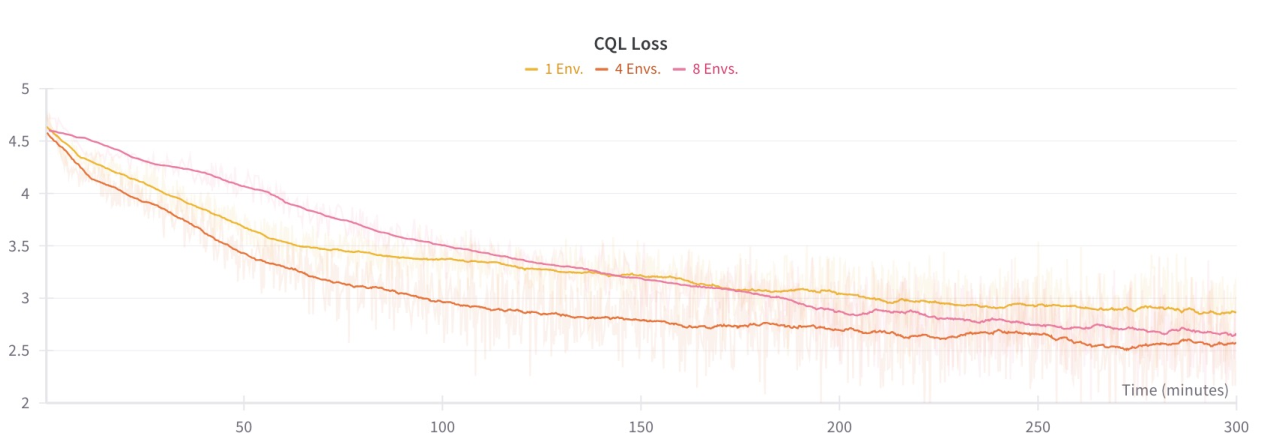
\includegraphics[width=1\linewidth]{image/offline_training_curve.pdf}
    \caption{The CQL loss curve during offline training with different offline datasets.}
    \label{fig:offline_curve}
\end{figure}



\begin{figure}[t]
    \centering
    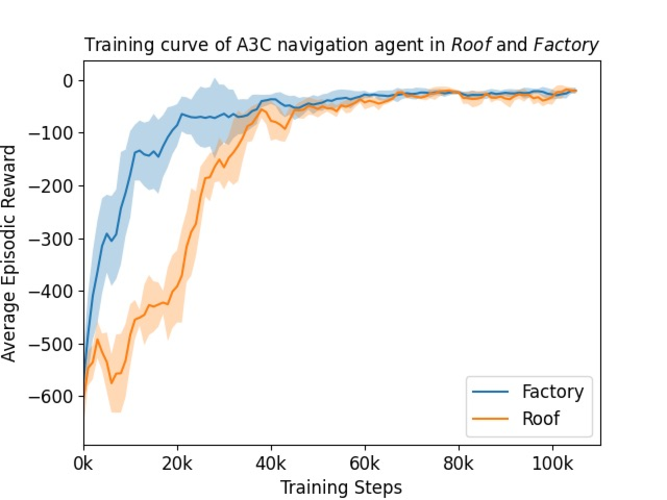
\includegraphics[width=0.6\linewidth]{image/training_curve.pdf}
    \caption{The learning curves for RL-based navigation agent in two environments: Roof and Factory. We use A3C~\citep{mnih2016asynchronous} to learn the navigation policy via trial-and-error interactions. In the Factory (blue line plot), the number of asynchronous workers is set to 4, while in the Roof environment (orange line plot), the number of asynchronous workers is set to 6. 
    }
    \label{fig:training_curve}
\end{figure}


\subsection{Evaluate Tracking Agents across 16 Unseen Environments}
\label{app:track16}
We provide the detailed quantitative evaluation results (episodic returns, episode length, success rate) of the RL-based embodied tracking agents across 16 environments, listed in Table~\ref{tab:eval_res}. In each environment, we report the average results over 50 episodes. The results show that in the \textit{Palace Maze}, which contains abundant structural obstacles, the agent's tracking performance was generally weaker compared to the other three categories. In contrast, the agent performed generally better in \textit{Lifelike Urbanity}, characterized by its relatively regular and flat terrain. Additionally, we observed that as the diversity of the training environments increased, the agent's tracking performance improved across all four environment categories. This highlights the positive impact of diverse training data on enhancing the agent's overall tracking effectiveness. We also provide vivid demo videos in \url{https://unrealzoo.notion.site/task-evt}.

\begin{table}[!t]
    \centering
    \caption{
    Quantitative evaluation results of the offline RL method across 16 environments. The environments are grouped into four categories: Compact Interior, Wildscape Realm, Palace Maze, and Lifelike Urbanity. The table compares the performance of agents trained on different offline dataset settings: 1 Env. (single environment), 2 Envs. (two environments), and 8 Envs. (eight environments). Each cell presents three metrics from left to right: Average Episodic Return (ER), Average Episode Length (EL), and Success Rate (SR). 
   }
   
\begin{tabular}{p{1.4cm}<{\centering}|c|ccc}
\hline
%\toprule
         Category &        Environment Name &  \tabincell{c}{1 Env. \\ ER/EL/SR} &  \tabincell{c}{2 Envs. \\ ER/EL/SR} &  \tabincell{c}{8 Envs. \\  ER/EL/SR} \\\hline
         %&&AR/EL/SR&AR/EL/SR&AR/EL/SR \\ \hline
%\midrule
\multirow{4}{*}{\tabincell{c}{Compact \\ Interior}} & Bunker & 241/412/0.56 &  245/391/0.56 &234/429/0.70    \\
                  & StorageHouse & 213 /424 /0.68 &275/449/0.76&170/434/0.64 \\
                  &  SoulCave & 229/402/0.60 &252/422/0.56&206/405/0.58 \\
                  & UndergroundParking & 179/391/0.56 &250/424/0.62&184/410/0.60  \\ \hline
\multirow{4}{*}{\tabincell{c}{Wildscape \\ Realm}} & Desert Ruins & 209/392/0.54 
                  &293/449/0.70&277/453/0.70\\
                  & GreekIsland & 245/411/0.62 &264/423/0.64
                 &257/466/0.78\\
                  & SnowMap & 204/399/0.62 &322/456/0.78 &278/474/0.86\\
                  & RealLandscape & 171 /383/0.42 &225/372/0.44&223/444/0.70 \\ \hline
\multirow{4}{*}{\tabincell{c}{Palace \\ Maze}} &  WesternGarden & 230/403/0.54 &  
                209/408/0.54&296/472/0.82 \\
                  & TerrainDemo & 232/411/0.56 & 233/403/0.56&192/411/0.56\\
                  & ModularGothicNight & 190/360/0.52 & 244/423/0.62&272/456/0.76\\
                  &ModularSciFiSeason1 & 168/365/0.42 &172/354/0.42&211/393/0.48\\ \hline
\multirow{4}{*}{\tabincell{c}{Lifelike \\ Urbanity}} &SuburbNeighborhoodDay & 224/422/0.64 &328/457/0.72&242/457/0.76\\
                  &DowntownWest & 296/460/0.78 &317/456/0.76		&292/469/0.86 \\
                  & Factory & 278/434/0.64 &291/452/0.74&249/435/0.64\\
                  & Venice & 295/441/0.70 &323/448/0.82&294/474/0.84\\ \hline
%\bottomrule
\end{tabular}
    % \end{threeparttable}
    % }
    % \vspace{-0.5cm}
    \label{tab:eval_res}
\end{table}

\begin{table}[tb]
    \centering
    \caption{
   Quantitative evaluation results of the tracking agents across 4 different category environments with \textbf{4 distractors (4D), 8 distractors (8D), and 10 distractors (10D)} respectively. The table compares the performance of agents trained on different offline dataset settings: 1 Env. (single environment), 2 Envs. (two environments), and 8 Envs. (eight environments). Each cell presents three metrics from left to right:  Average Episodic Return (ER), Average Episode Length (EL), and Success Rate (SR).
   }
    % \vspace{-0.3cm}
    % \resizebox{1\linewidth}{!}{
    % \begin{threeparttable}
\begin{tabular}{p{1.4cm}<{\centering}|c|ccc}
\hline
%\toprule
         Category &        Environment Name &  \tabincell{c}{1 Env. \\ ER/EL/SR} &  \tabincell{c}{2 Envs. \\ ER/EL/SR} &  \tabincell{c}{8 Envs. \\  ER/EL/SR} \\ \hline
         %&&AR/EL/SR&AR/EL/SR&AR/EL/SR \\ \hline
%\midrule
\multirow{3}{*}{\tabincell{c}{Compact \\ Interior}} &           StorageHouse (4D)& 117/343/0.40 & 181/375/0.52   &190/428/0.62\\
&           StorageHouse (8D)& 143/341/0.34 & 151/338/0.44   &165/366/0.49\\
                  & StorageHouse (10D)& 81/324/0.36 &109/331/0.42& 107/357/0.50\\ \hline
                 
\multirow{3}{*}{\tabincell{c}{Wildscape \\ Realm}} 
                    & DesertRuins (4D)& 317/469/0.72
                  &333/456/0.70&354/466/0.74\\ 
                  & DesertRuins (8D)& 213/406/0.50
                  &316/445/0.58&267/444/0.68\\
                  & DesertRuins (10D)& 188/390/0.44 
                  &252/382/0.50&253/447/0.64\\
                  \hline
\multirow{3}{*}{\tabincell{c}{Palace \\ Maze}} &  TerrainDemo (4D)&  221/398/0.44 & 286/454/0.65 & 312/460/0.77 \\
&  TerrainDemo (8D)& 211/384/0.39 & 239/412/0.49 & 252/420/0.52 \\
                  & TerrainDemo (10D)& 189/377/0.36 & 232/404/0.48&224/429/0.66\\
                  \hline

\multirow{3}{*}{\tabincell{c}{Lifelike \\ Urbanity}} 
&SuburbNeighborhoodDay (4D)     
  &192/407/0.46&256/381/0.50&265/392/0.60\\
  &SuburbNeighborhoodDay (8D)     
  &131/325/0.36&229/369/0.48&247/385/0.56\\
&SuburbNeighborhoodDay (10D)     
  &162/355/0.44&180/340/0.40&165/376/0.44\\
                 \hline

%\bottomrule
\end{tabular}
    % \end{threeparttable}
    % }
    % \vspace{-0.5cm}
    \label{tab:eval_dis}
\end{table}

\subsection{Evaluate Tracking Agents across Unseen Social Environments}
\label{app:social}

We select 4 environments from different categories as the testing environments, including StorageHouse, DesertRuins, TerrainDemo, and SurburNeighborhoodDay. We test the distraction robustness of the social tracking agents by adding different numbers of distractors (4, 8, 10) in the environment. The distractors randomly walk around the environment, which may produce various unexpected perturbations to the tracker, such as visual distractions, occlusion, or blocking the tracker's path. As shown in Table~\ref{tab:eval_dis}, the tracking performance of the three agents steadily decays with the increasing number of distractors.



% Distractor experiment
% \begin{table}[!t]
%     \centering
%     \caption{
%    Quantitative evaluation results of the tracking agents across 16 environments with \textbf{10 distractors (10D)}. The table compares the performance of agents trained on different offline dataset
% settings: 1 Env. (single environment), 2 Envs. (two environments), and 8 Envs. (eight environments).
% Each cell presents three metrics from left to right: Average Accumulated Reward (AR), Average
% Episode Length (EL), and Success Rate (SR)
%    }
%     % \vspace{-0.3cm}
%     % \resizebox{1\linewidth}{!}{
%     % \begin{threeparttable}
% \begin{tabular}{p{1.4cm}<{\centering}|c|ccc}
% \hline
% %\toprule
%          Category &        Environment Name &  \tabincell{c}{1 Env. \\ AR/EL/SR} &  \tabincell{c}{2 Envs. \\ AR/EL/SR} &  \tabincell{c}{8 Envs. \\  AR/EL/SR} \\ \hline
%          %&&AR/EL/SR&AR/EL/SR&AR/EL/SR \\ \hline
% %\midrule
% \multirow{5}{*}{\tabincell{c}{Compact \\ Interior}} &           Bunker (10D)& -14/235/0.10 &  98/324/0.24 &54/252/0.12\\
%                   & StorageHouse (10D)& 81/324/0.36 &109/331/0.42& 107/357/0.50\\
%                   &  SoulCave (10D) & 132/337/0.38 &183/380/0.50& 123/371/0.48\\
%                   & UndergroundParking (10D)& -32/224/0.04 &106/313/0.18 &120/365/0.21  \\ \hline 
%                   &Mean &42/280/0.22&124/337/0.36&101/336/0.33\\ \hline
% \multirow{5}{*}{\tabincell{c}{Wildscape \\ Realm}} & DesertRuins (10D)& 188/390/0.44 
%                   &252/382/0.50&253/447/0.64\\
%                   & GreekIsland (10D)& 173/389/0.48 &288/419/0.60
%                  &233/418/0.56\\
%                   & SnowMap (10D)& 240/429/0.60&305/429/0.68 &208/418/0.58\\
%                   & RealLandscape (10D)& 111/343/0.34 &211/370/0.42&112/371/0.36 \\ \hline 
%                 &Mean &178/388/0.47&264/400/0.55&201/414/0.54\\ \hline
% \multirow{5}{*}{\tabincell{c}{Palace \\ Maze}} &  WesternGarden (10D)&195/365/0.5 & 175/348/0.42 &175/360/0.42
%                  \\
%                   & TerrainDemo (10D)& 189/377/0.36 & 232/404/0.48&224/429/0.66\\
%                   & ModularGothicNight (10D)&35/269/0.12  & 87/324/0.20&71/359/0.28\\
%                   &ModularSciFiSeason1 (10D)& 95/304/0.28 &151/323/0.36&123/342/0.38\\ \hline
%                 &Mean &129/329/0.32&161/350/0.37&148/373/0.44\\ \hline

% \multirow{5}{*}{\tabincell{c}{Lifelike \\ Urbanity}} &SuburbNeighborhoodDay (10D)     
%   &162/355/0.44&180/340/0.4&165/376/0.44\\
%                   &DowntownWest (10D)& 230/247/0.64&258/428/0.68		&218/444/0.68 \\
%                   & Factory (10D)& 75/300/0.30&141/339/0.40&107/322/0.32\\
%                   & Venice (10D)& 158/369/0.38&295/435/0.68&177/376/0.54\\ \hline
%                 &Mean &156/318/0.44&219/386/0.54&167/380/0.50\\ \hline

% %\bottomrule
% \end{tabular}
%     % \end{threeparttable}
%     % }
%     % \vspace{-0.5cm}
%     \label{tab:eval_res}
% \end{table}







